\documentclass[11pt]{article}

\usepackage{pdp}

%------------------------------------------------------------------------------
%	REPORT INFORMATION
%------------------------------------------------------------------------------

\title{Carcassonne -- Python}
\subtitle{Rapport préliminaire}
\author{Anthony BEAUVIEUX, Tony HUANG, Maxence SALIN, Clément SIMON, Loïc THIN}
\date{}

%------------------------------------------------------------------------------

\begin{document}

%------------------------------------------------------------------------------
%	TITLE PAGE
%------------------------------------------------------------------------------

\maketitle
\thispagestyle{empty}

%------------------------------------------------------------------------------
%	MAIN MATTER
%------------------------------------------------------------------------------

\section{Présentation du jeu}

\subsection{Existant}

\textbf{Carcassonne} est un jeu de stratégie et de placement de tuiles créé par Klaus-Jürgen Wrede en 2000, conçu pour 2 à 6 joueurs.
Il s'agit d'un jeu stochastique à information parfaite, c'est-à-dire un jeu où le hasard intervient dans le tirage des tuiles mais où l'ensemble des éléments présents sur le plateau est visible de tous les joueurs.

Le jeu a connu un succès commercial important donnant lieu à de nombreuses extensions et variantes au fil des années. Il est devenu un classique des jeux de société modernes, alliant stratégie, gestion de ressources et placement de tuiles. Sur le plan académique et technique, Carcassonne représente un terrain d'étude privilégié pour l'intelligence artificielle (IA) et les algorithmes de décision, en raison de sa nature stochastique, de son système de scoring complexe et de la diversité des stratégies possibles. Plusieurs travaux académiques et implémentations logicielles ont étudié les problématiques liées à l'intelligence artificielle pour Carcassonne. L'article de Heyden et al.\cite{heyden2009implementing} propose une analyse détaillée de l'arbre de jeu et des techniques de recherche heuristique adaptées aux contraintes de ce jeu, tandis que d'autres études explorent des approches basées sur Monte Carlo ou Expectimax pour gérer l'incertitude liée à la pioche des tuiles.


\subsection{Contexte}

\begin{wrapfigure}{l}{0.25\textwidth}
  \centering
  \captionsetup{justification=centering}
    \frame{
\includegraphics[width=0.1\textwidth]{images/carcassonne_starting_tile.png}}
    \caption{Tuile de départ}\label{fig:tuile_de_départ}
  \end{wrapfigure}

La version considérée ici utilise les 72 tuiles du jeu de base.
Parmi ces tuiles, se trouve la tuile de départ (figure \ref{fig:tuile_de_départ}) qui est placée au centre du plateau avant le début de la partie. 
Cette tuile est la même pour chaque partie et comporte une \textit{City} en haut (couleur marron), une \textit{Road} qui traverse la tuile de gauche à droite et un \textit{Field} en bas.
Chaque joueur dispose de 7 pions de sa couleur pour marquer des points au cours de la partie.
Le but du jeu est que les joueurs construisent progressivement le plateau, à tour de rôle, en posant des tuiles de manière cohérente et en plaçant stratégiquement leurs pions pour accumuler des points.
Le vainqueur est le joueur qui totalise le plus de points à la fin de la partie.
\subsection{Règles}

Les règles de \textbf{Carcassonne} utilisées sont celles de la version 2012\cite{rulescarcassonne}.

\subsubsection{Spécificités}
\begin{description}[style=nextline]
  \item[Tuile] Chaque tuile possède quatre côtés ainsi qu'un centre.
  Chaque côté correspond à un type de terrain parmi \textit{Road}, \textit{City} ou \textit{Field}.
  Le centre peut représenter une \textit{City}, un \textit{Field}, une \textit{Banner} ou un \textit{Monastery}.
  \begin{figure}[H]
    \centering
    \captionsetup{justification=centering}
    
  \begin{minipage}{0.35\textwidth}
    \centering
    \frame{
\includegraphics[width=0.20\textwidth]{images/carcassonne_example_tile_monastery.png}}
    \caption{Exemple d'une tuile où des \textit{Fields} possèdent un \textit{Monastery}}\label{fig:exemple_tuile_1}
  \end{minipage}
  \hspace{0.5cm}
 \begin{minipage}{0.35\textwidth}
    \centering
    \frame{
\includegraphics[width=0.20\textwidth]{images/carcassonne_example_tile_banner.png}}
    \caption{Exemple d'une tuile où une \textit{City} possède une \textit{Banner}}\label{fig:exemple_tuile_2}
  \end{minipage}
  
  \end{figure}

  \item[Pion] Lorsqu'un pion est placé sur une tuile, il prend un rôle en fonction du type de terrain occupé :
  \textit{Knight} sur une \textit{City}, \textit{Farmer} sur un \textit{Field}, \textit{Thief} sur une \textit{Road}
  et \textit{Monk} sur un \textit{Monastery}.
\end{description}



\subsubsection{Déroulement d'un tour}

Les joueurs jouent à tour de rôle selon un ordre prédéfini (généralement dans le sens horaire, en commençant par le joueur le plus jeune). 
Lors de son tour, un joueur effectue les actions suivantes dans l'ordre indiqué :

\begin{enumerate}
  \item \textbf{Piocher une tuile :}  
  Le joueur pioche une tuile dans la pioche actuellement active. Cette tuile est visible par l'ensemble des joueurs.

  \item \textbf{Placer la tuile :}  
  La tuile piochée doit être placée sur le plateau en respectant les règles suivantes :
  \begin{itemize}
    \item[-] La tuile doit être adjacente à au moins une autre tuile déjà posée.
    \item[-] Les côtés en contact doivent correspondre à des terrains de même type.
  \end{itemize}

  \item \textbf{Placer un pion (optionnel) :}  
  Le joueur peut placer un pion sur un élément de terrain de la tuile qu'il vient de poser (\textit{City}, \textit{Road}, \textit{Field}, \textit{Monastery}).

  \item \textbf{Restriction de placement des pions :}  
  Si l'élément de terrain choisi est relié à un élément du même type déjà occupé par un pion, aucun nouveau pion ne peut y être placé.
  Les \textit{Road} et \textit{City} agissent comme des séparateurs entre les \textit{Field}.

  \item \textbf{Résolution des terrains complétés :}  
  Si la pose de la tuile permet de compléter un ou plusieurs terrains, ceux-ci sont résolus immédiatement et les joueurs concernés marquent des points selon certaines règles. (voir partie \ref{subsubsec:score})

  \item \textbf{Retour des pions :}  
  Tous les pions associés à des \textit{City}, \textit{Road} ou \textit{Monastery} complétés durant le tour actuel sont retirés du plateau et rendus à leurs propriétaires. Les pions \textit{Farmer} restent en jeu jusqu'à la fin de la partie.

\end{enumerate}

\subsubsection{Score}
\label{subsubsec:score}
Les points sont attribués à deux moments :
\begin{itemize}
  \item[$\bullet$] Pendant la partie : dès qu'un terrain  (\textit{City}, \textit{Road}, \textit{Monastery}) est complété (figure \ref{fig:example_tour}).
  \item[$\bullet$] À la fin de la partie : pour les terrains incomplets (\textit{City}, \textit{Road}, \textit{Monastery}) ainsi que pour les \textit{Field}.
\end{itemize}

Les joueurs ajoutent alors à leur score les points correspondant aux terrains selon les règles suivantes :

  \begin{description}[style=nextline]
  \item[ \textcolor{gray}{Road} :]
  Une \textit{Road} rapporte 1 point par tuile la composant au joueur possédant le plus de pions (\textit{Thief}) sur cette \textit{Road}.
  En cas d'égalité, tous les joueurs concernés marquent ces points.

  \item[ \textcolor{brown}{City} :]
  Une \textit{City} complète rapporte 2 points par tuile qui la compose ainsi que 2 points par \textit{Banner} présent,
  pour le joueur possédant le plus de pions (\textit{Knight}). Si la \textit{City} est incomplète à la fin de la partie, chaque tuile rapporte 1 point et chaque \textit{Banner} rapporte également 1 point.
  En cas d'égalité, les points sont attribués à tous les joueurs concernés.

  \item[ \textcolor{red}{Monastery} :]
  Un \textit{Monastery} rapporte 1 point par tuile ayant un sommet ou côté en commun, y compris la tuile du \textit{Monastery}. Le score maximal d'un \textit{Monastery} est donc de 9 points.

  \item[ \textcolor{green}{Field} :]
  Chaque ensemble de \textit{Fields} connectés ou isolés est attribué au joueur possédant le plus de pions (\textit{Farmer}).
  Il marque alors 3 points par \textit{City} complète adjacente aux \textit{Field}.
  En cas d'égalité, tous les joueurs concernés marquent ces points.
\end{description}

A l'issue du décompte final, le joueur ayant obtenu le plus grand nombre de points remporte la partie.
\begin{figure}[H]
    \centering
    \captionsetup{justification=centering}
    \frame{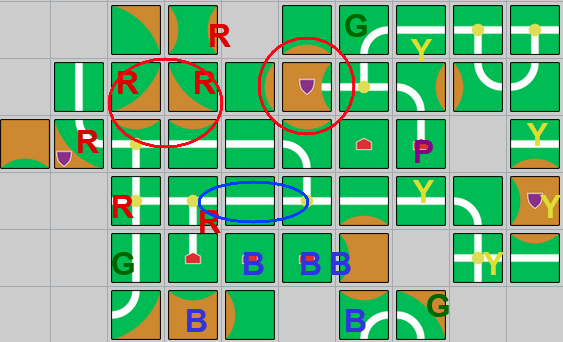
\includegraphics[width=0.60\textwidth]{images/carcassonne_exemple_partie_complete.png}}
    \centering
    \caption{Exemple de terrains complétés, avec deux \textit{City} entourées en rouge et une \textit{Road} entourée en bleu}\label{fig:example_tour}
\end{figure}


\subsection{Complexité}

Bien que les règles de \textbf{Carcassonne} soient relativement simples, le jeu présente une richesse stratégique importante qui augmente à mesure que le plateau s'étend. 
Les choix offerts aux joueurs se multiplient progressivement en fonction de la configuration du plateau, des tuiles restantes et du placement des pions.

Contrairement à des jeux déterministes comme les échecs ou le shogi, \textbf{Carcassonne} introduit une composante stochastique via la pioche des tuiles, ce qui complexifie l'anticipation des coups futurs. 
Néanmoins, il demeure un jeu à information parfaite dans la mesure où l'ensemble des éléments placés sur le plateau est visible par tous les joueurs à tout instant.

La complexité combinatoire du jeu est particulièrement élevée pour plusieurs raisons. D'abord, chaque tuile peut être orientée de quatre manières, et chaque position libre sur le plateau peut être un emplacement légitime lorsque les côtés adjacents correspondent. Ensuite, la taille effective de l'espace d'états dépend de l'ordre de tirage des 72 tuiles, du placement des meeples et de la résolution des structures incomplètes. Sur un plateau en croissance, le nombre de successeurs possibles à un instant donné peut rapidement dépasser plusieurs dizaines, ce qui conduit à un arbre de jeu de taille astronomique. La taille de l'arbre de jeu est estimée à environ $10^{194}$\cite{heyden2009implementing}, ce qui rend toute exploration exhaustive irréaliste.

Mathématiquement, ce type de complexité se situe entre la simple permutation des tuiles et un vaste graphe de configurations : il faut combiner 72 choix de tuiles avec 4 orientations possibles et un grand nombre de positions valides, d'où un nombre de branches extrêmement élevé. D'où la nécessité d'un compromis entre profondeur de recherche, précision des heuristiques et temps de calcul.

Dans ce contexte, l'utilisation d'algorithmes de recherche heuristique et d'approximation apparaît comme une solution nécessaire pour proposer des décisions pertinentes dans un temps de calcul raisonnable.



\section{Algorithmes et structures de données}

Dans le cadre de ce projet, \textbf{Carcassonne} est considéré sous une forme restreinte pour la partie de réalisation d'intelligence artificielle afin de rendre possible l'utilisation d'algorithmes classiques de recherche dans les jeux.

Bien que \textbf{Carcassonne} ne soit pas strictement un jeu à somme nulle et qu'il comporte une composante stochastique liée à la pioche des tuiles, certaines hypothèses simplificatrices sont adoptées.
En particulier, les décisions sont évaluées à partir de fonctions heuristiques estimant l'avantage relatif d'un joueur par rapport à son adversaire à un instant donné.

Cette modélisation permet l'utilisation d'algorithmes de recherche tels que Minimax et ses variantes, tout en restant consciente des limites théoriques de leur application à un jeu de cette nature.

Plusieurs algorithmes jouent ainsi un rôle central dans la réalisation des besoins du projet, notamment :
\begin{itemize}
  \item[-] \textbf{Minimax}\cite{minimax}, pour déterminer les coups optimaux en modélisant l'opposition entre les joueurs ;
  \item[-] \textbf{Alpha-Beta}\cite{alpha_beta}, qui permet de réduire le nombre d'états explorés en élaguant les branches non pertinentes de l'arbre de jeu ;
  \item[-] \textbf{Iterative Deepening}\cite{iterative_deepening}, utilisé afin de borner le temps de calcul tout en améliorant progressivement la qualité des décisions ;
  \item[-] \textbf{des fonctions d'évaluation heuristiques}, servant à estimer la qualité d'un état de jeu ;
  \item[-] des approches basées sur \textit{Monte Carlo Tree Search}\cite{monte_carlo}, envisagées pour des stratégies alternatives ;
  \item[-] des algorithmes de génération aléatoire, tels que le mélange de \textit{Fisher–Yates}\cite{fisher_yates}, nécessaires à la gestion équitable de la pioche.
\end{itemize}

La mise en œuvre efficace de ces algorithmes repose sur des structures de données adaptées permettant de représenter l'état du jeu et d'en faciliter la manipulation. 
Le plateau de jeu, constitué de tuiles connectées par leurs côtés, est modélisé en interne par un graphe de positions, offrant une représentation naturelle des relations d'adjacence entre les tuiles. 
Les états de jeu sont stockés sous forme d'objets si bien que chaque tuile possède un identifiant, un jeu de côtés, une rotation et des informations sur les meeples attachés.

La gestion de la pioche et du retour des pions utilise des structures séquentielles simples, comme des listes et des piles. Pour les calculs de score et la recherche de composantes connexes, des parcours en largeur (BFS) sur le graphe de tuiles sont employés, avec des ensembles de sommets visités pour éviter les redondances.

\subsection{Structures de données}

La représentation des données du jeu est un point clé du projet. En Python, le plateau est principalement géré par un dictionnaire de positions vers les tuiles, complété par une table d'adjacence pour les voisinages.

{\normalsize
  \begin{minted}[frame=single]{python}
class Tile:
    code: str

    # Direction matrices indexed by orientation (0, 1, 2, 3)
    direction_matrix = [
        # 0 rotation
        [["NW", "N", "NE"], ["W", "C", "E"], ["SW", "S", "SE"]],
        # 1 rotation (90° clockwise)
        [["SW", "W", "NW"], ["S", "C", "N"], ["SE", "E", "NE"]],
        # 2 rotations (180° clockwise)
        [["SE", "S", "SW"], ["E", "C", "W"], ["NE", "N", "NW"]],
        # 3 rotations (270° clockwise)
        [["NE", "E", "SE"], ["N", "C", "S"], ["NW", "W", "SW"]],
    ]

    def __init__(
        self,
        code: str,
        connections: dict | None = None,
        connect_to: dict | None = None,
    ) -> None:
        self.code = code
        # tiles_lands is the terrain definitions for this tile
        self.tiles_lands = connections if connections is not None else {}
        self.connect_to = connect_to if connect_to is not None else {}
  \end{minted}
}

Cette structure permet de calculer rapidement les composantes connexes nécessaires au calcul des champs, des routes et des cités.

Les états de partie sont ensuite définis par une classe `GameState` contenant le plateau, la pioche restante, les scores et le nombre de meeples disponibles par joueur.

\subsection{Mélange des tuiles}

La gestion de la pioche repose sur deux algorithmes de mélange. L'algorithme principal retenu est \textit{Fisher–Yates}\cite{fisher_yates}, car il produit une permutation uniforme des tuiles lorsqu'il est associé à un générateur pseudo-aléatoire uniforme. En parallèle, nous conservons également un algorithme naïf, utilisé comme point de comparaison expérimental afin d'illustrer les biais possibles d'un mauvais mélange.

Les deux implémentations sont réalisées \textit{in place} sur la liste représentant la pioche :

{\normalsize
  \begin{minted}[frame=single]{python}
import random

@staticmethod
def _shuffle_fisher_yates_in_place(
    items: list[str], rng: random.Random
) -> None:
    for i in range(len(items) - 1, 0, -1):
        j = rng.randrange(i + 1)
        items[i], items[j] = items[j], items[i]

@staticmethod
def _shuffle_naive_in_place(items: list[str], rng: random.Random) -> None:
    n = len(items)
    for i in range(n):
        j = rng.randrange(n)
        items[i], items[j] = items[j], items[i]
  \end{minted}
}

Dans la pratique, \textit{Fisher–Yates} est utilisé par défaut pour garantir une pioche équitable, tandis que l'algorithme naïf est conservé à des fins de test et de comparaison.

Dans la suite de cette section, nous nous concentrerons plus particulièrement sur les quatre premiers algorithmes présentés qui constituent le cœur du système de prise de décision implémenté dans le projet.

\subsection{Algorithme Minimax}
\label{subsec:minimax}

L'algorithme Minimax a pour but de déterminer les coups les plus optimaux pour un joueur à un état donné du jeu face à l'adversaire qui minimise le score du joueur "max".
Ainsi, l'algorithme parcourt récursivement une partie de l'arbre des états du jeu, limitée par une profondeur maximale fixée afin de contenir la complexité de recherche.
Chaque score d'une feuille est alors calculé via une fonction d'évaluation prédéfinie. Ce score remonte à son nœud parent qui sélectionne la valeur maximale ou minimale de ses nœuds enfants selon le joueur qu'il représente, et ainsi de suite jusqu'à la racine.
L'algorithme possède 3 paramètres représentant l'état du jeu courant, la profondeur restante à explorer par rapport à l'état actuel, et un booléen à vrai lors du tour du joueur "max" et à faux sinon.

Voici le pseudocode de l'algorithme Minimax :
{\normalsize
  \begin{minted}[frame=single]{text}
fonction minimax(etat, profondeur, joueur_max):
    SI profondeur = 0 OU estFeuille(etat) ALORS
        RETOURNER evalueHeuristique(joueur_max, etat)
    FIN SI
    SI joueur_max ALORS
        valeur = -infini
        POUR TOUT successeur s de etat FAIRE
            valeur = max(valeur, minimax(s, profondeur - 1, FAUX))
        FIN POUR TOUT
    FIN SI
    SINON
        valeur = +infini
        POUR TOUT successeur s de etat FAIRE
            valeur = min(valeur, minimax(s, profondeur - 1, VRAI))
        FIN POUR TOUT
    FIN SINON
    RETOURNER valeur
FIN FONCTION

  \end{minted}
}


\begin{figure}[H]
    \centering
    \captionsetup{justification=centering}
    \frame{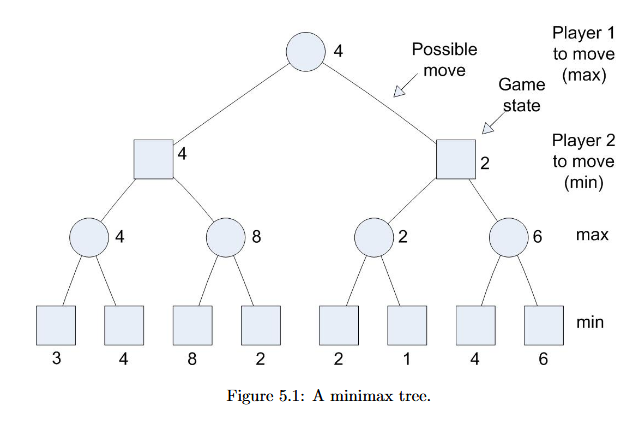
\includegraphics[width=0.60\textwidth]{images/minimax.png}}
    \centering
    \caption{Exemple d'un arbre de jeu partiel exploré par l'algorithme Minimax\cite{heyden2009implementing}}\label{fig:minimax_example}
\end{figure}

À la profondeur maximale à explorer, les feuilles remontent la valeur 4 (et non la valeur 3) lors du tour du joueur "max" pour maximiser son gain. 
Ainsi, au tour suivant, le joueur "min" récupère cette valeur 4 (et non la valeur 8) afin de minimiser le gain de son adversaire. 
Enfin, le joueur "max" récupère la valeur 4 (et non la valeur 2) pour maximiser son gain minimal. 
Il finit alors la recherche à la racine de l'arbre, ayant désormais connaissance d'une succession de coups optimaux à jouer pour obtenir un score de 4 en sa faveur à cette profondeur demandée.

\subsection{Technique Iterative Deepening}

L'algorithme Minimax avec approfondissement itératif (Iterative Deepening) est une technique de parcours progressif des profondeurs sur l'arbre des états d'un jeu. 
Après un parcours avec une nouvelle profondeur explorée, le meilleur coup pour le joueur "max" est enregistré en remplaçant le précédent, et sera alors renvoyé après épuisement du temps donné. 
Cette technique a pour avantage de déterminer une solution utile même sur une courte durée, tandis que l'exploration classique ne garantit pas que la profondeur fixée soit suffisante pour obtenir un résultat fiable après un temps bloquant.

En pratique, la recherche commence à faible profondeur puis augmente progressivement jusqu'à atteindre le temps limite :
{\normalsize
  \begin{minted}[frame=single]{text}
fonction choix_coup(etat, temps_max):
    profondeur = 1
    meilleur_coup = null
    debut = temps()
    TANT_QUE temps() - debut < temps_max FAIRE
        meilleur_coup = recherche_minimax(etat, profondeur)
        profondeur += 1
    FIN TANT_QUE
    RETOURNER meilleur_coup
FIN FONCTION
  \end{minted}
}

Cette approche garantit qu'un coup plausible est toujours disponible à la fin du délai, même si la profondeur maximale n'a pas pu être atteinte.

\subsection{Algorithme Alpha-Beta}

Alpha-Beta (ou $\alpha\beta$-pruning) est une variante de l'algorithme Minimax consistant à explorer partiellement l'arbre des états d'un jeu en élaguant les branches qui n'apportent aucun gain nouveau pour le joueur "max".\cite{alpha_beta}
En stockant la meilleure valeur courante pour le joueur maximal ($\alpha$) et celle pour le joueur "min" ($\beta$) lors du parcours, l'algorithme n'évalue plus certains nœuds non-significatifs (et leurs potentiels enfants) quand $\alpha \geq \beta$, en réduisant potentiellement son temps d'exécution selon l'arbre donné.

Le principe est le suivant : dès qu'une branche devient trop mauvaise pour l'un des joueurs, elle ne peut plus influencer la décision finale et peut être abandonnée. Le gain en temps est particulièrement important lorsque les successeurs sont ordonnés de manière à évaluer d'abord les coups les plus prometteurs.

{\normalsize
  \begin{minted}[frame=single]{text}
fonction alpha_beta(etat, profondeur, alpha, beta, joueur_max):
    SI profondeur = 0 OU estFeuille(etat) ALORS
        RETOURNER evalueHeuristique(etat)
    FIN SI
    SI joueur_max ALORS
        valeur = -infini
        POUR TOUT successeur s de etat FAIRE
            valeur = max(valeur, alpha_beta(s, profondeur - 1, alpha, beta, FAUX))
            alpha = max(alpha, valeur)
            SI alpha >= beta ALORS
                BRISER
            FIN SI
        FIN POUR TOUT
    SINON
        valeur = +infini
        POUR TOUT successeur s de etat FAIRE
            valeur = min(valeur, alpha_beta(s, profondeur - 1, alpha, beta, VRAI))
            beta = min(beta, valeur)
            SI beta <= alpha ALORS
                BRISER
            FIN SI
        FIN POUR TOUT
    FIN SINON
    RETOURNER valeur
FIN FONCTION
  \end{minted}
}

Cette version conserve la qualité de la décision de Minimax, tout en réduisant significativement le nombre de nœuds évalués lorsque le tri des coups est efficace.

\subsection{Fonction d'évaluation heuristique}

Étant donné l'impossibilité d'explorer l'arbre de jeu jusqu'à des états terminaux, l'algorithme Minimax repose sur une fonction d'évaluation heuristique permettant d'estimer la qualité d'un état de jeu intermédiaire.
Cette fonction associe une valeur numérique à un état donné, représentant l'avantage relatif du joueur courant par rapport à son adversaire.

L'évaluation repose notamment sur les critères suivants :
\begin{itemize}
  \item [$\bullet$] le score actuel des joueurs ;
  \item [$\bullet$] le potentiel de complétion des routes, cités et monastères en cours ;
  \item [$\bullet$] le nombre de pions disponibles pour chaque joueur ;
  \item [$\bullet$] la présence de pions bloqués sur des structures difficilement complétables ;
  \item [$\bullet$] le contrôle des champs adjacents à des cités complètes.
\end{itemize}

Ces différents éléments sont pondérés afin de refléter leur importance stratégique au cours de la partie.
La fonction d'évaluation ne prétend pas fournir une estimation parfaite, mais permet de guider efficacement la recherche vers des coups jugés prometteurs.

\subsection{Lien avec le projet}

Les différentes techniques sont combinées dans le projet afin de rendre la recherche de coups pertinents possible malgré la complexité combinatoire élevée de Carcassonne. 
L'approche adoptée, mêlant Minimax, élagage Alpha-Beta, approfondissement itératif et fonctions d'évaluation heuristique, permet de guider efficacement la prise de décision des intelligences artificielles tout en respectant des contraintes de temps réalistes.
La modélisation du plateau sous forme de graphes, associée à l'utilisation de structures de données adaptées comme les tables de hachage et les piles, assure une manipulation efficace de l'état du jeu et des configurations intermédiaires.

Ainsi, bien que l'exploration exhaustive de l'arbre de jeu reste impossible, le système mis en place fournit des conseils et des stratégies de qualité, exploitant de manière pragmatique les ressources computationnelles disponibles. 
Cette combinaison d'algorithmes et de structures de données constitue le cœur de l'intelligence artificielle du projet et offre une base solide pour l'extension future des fonctionnalités, telles que l'intégration de stratégies plus sophistiquées ou de variantes du jeu.



\section{Architecture}
Dans cette section, nous présentons l'architecture logicielle retenue pour l'implémentation du jeu Carcassonne.
Le projet adopte une architecture n-tiers\cite{n_tier_architecture} visant à séparer clairement les responsabilités afin d'améliorer la maintenabilité, la testabilité et l'évolutivité du code.
Le principe fondamental de cette architecture est de diviser le système en couches distinctes, chacune ayant des responsabilités spécifiques, et de limiter les dépendances au minimum grâce à des interfaces bien définies.

Dans un modèle n-tiers classique, chaque couche n'utilise que les services exposés par la couche située en dessous d'elle et ne dépend pas des détails d'implémentation de cette couche. Cela permet, par exemple, de remplacer l'interface utilisateur (CLI ou GUI) sans toucher à la logique métier, ou de simuler la persistance en tests unitaires en fournissant un faux service de stockage.

Ainsi, dans notre projet, nous avons choisi une architecture à trois tiers avec une séparation nette entre la présentation, la logique métier et les données.
Cette architecture est pertinente dans notre cas car elle permet de faire évoluer le jeu sans mélanger les règles du jeu, l'affichage et la persistance des données. Elle est structurée autour de trois modules principaux : Présentation, Logique Métier et Données, organisés selon des dépendances unidirectionnelles.

\subsection{Découpage en modules}

\begin{tcolorbox}[
  colback=gray!5,
  colframe=black,
  boxrule=0.8pt,
  arc=2mm
]
\large\textbf{Module Présentation}\normalsize
\vspace{0.3em}

Le module Présentation est responsable des interactions avec l'utilisateur et de l'affichage de l'état du jeu.
Il comprend notamment la gestion des commandes à travers le shell en CLI ou des actions à partir de la GUI, l'affichage du plateau, des tuiles, des meeples et des scores à travers CLI ou GUI.

Ce module ne contient aucune règle métier. Il délègue toute décision concernant la validité des actions ou l'évolution du jeu au module Logique Métier.

\vspace{0.5em}
\textbf{Responsabilités principales :}
\begin{itemize}
  \item[$\bullet$] Interprétation des actions utilisateur


  \item[$\bullet$] Appels aux interfaces de la logique métier


  \item[$\bullet$] Rafraîchissement de l'affichage
\end{itemize}

\medskip
\hrule
\medskip

\large\textbf{Module Logique Métier}\normalsize
\vspace{0.3em}

Le module Logique Métier constitue le cœur du jeu.
Il encapsule l'ensemble des règles du jeu et gère l'état interne de la partie.
Il est notamment responsable de la mise à jour du plateau (via une liste d'adjacence), du calcul des scores, de la gestion des tours de jeu et des conditions de fin de partie. 
Il prend également en charge les actions des intelligences artificielles, à l'aide de fonctions d'évaluation, ainsi que la gestion de l'état du serveur et des parties en cours.

Ce module est totalement indépendant de l'interface graphique et de la persistance.

\vspace{0.5em}
\textbf{Responsabilités principales :}

\begin{itemize}
  \item[$\bullet$] Implémentation des règles du jeu 
  \item[$\bullet$] Gestion de l'état de la partie 
  \item[$\bullet$] Gestion des IA de jeu 
  \item[$\bullet$] Gestion des actions liées au serveur
\end{itemize}


\medskip
\hrule
\medskip

\large\textbf{Module Données}\normalsize
\vspace{0.3em}

Le module Données est dédié à la persistance et à la gestion des informations liées au jeu.
Il s'occupe de la sauvegarde et du chargement des parties, de l'enregistrement de l'historique de jeu, ainsi que de la conservation des données relatives aux intelligences artificielles, notamment les structures de données et les meilleurs coups mémorisés dans le cadre de l'iterative deepening.
Il gère également la persistance des parties en cours, de l'état du serveur et des informations associées aux joueurs.

Ce module n'implémente aucune règle métier et n'interagit jamais directement avec l'interface utilisateur.

\vspace{0.5em}
\textbf{Responsabilités principales :}
\begin{itemize}
  \item[$\bullet$] Sauvegarde des informations liées au jeu de près ou de loin (avec IA et serveurs) ;
  \item[$\bullet$] Possibilité de sauvegarder les parties en cours pour les recharger (dans des fichiers au format répondant aux fonctionnalités).
\end{itemize}

\end{tcolorbox}

\subsection{Dépendances entre modules}
Les dépendances entre modules sont strictement unidirectionnelles (figure \ref{fig:UML_diagram}), conformément au principe d'architecture N-tiers.
\begin{figure}[H]
    \centering
    \frame{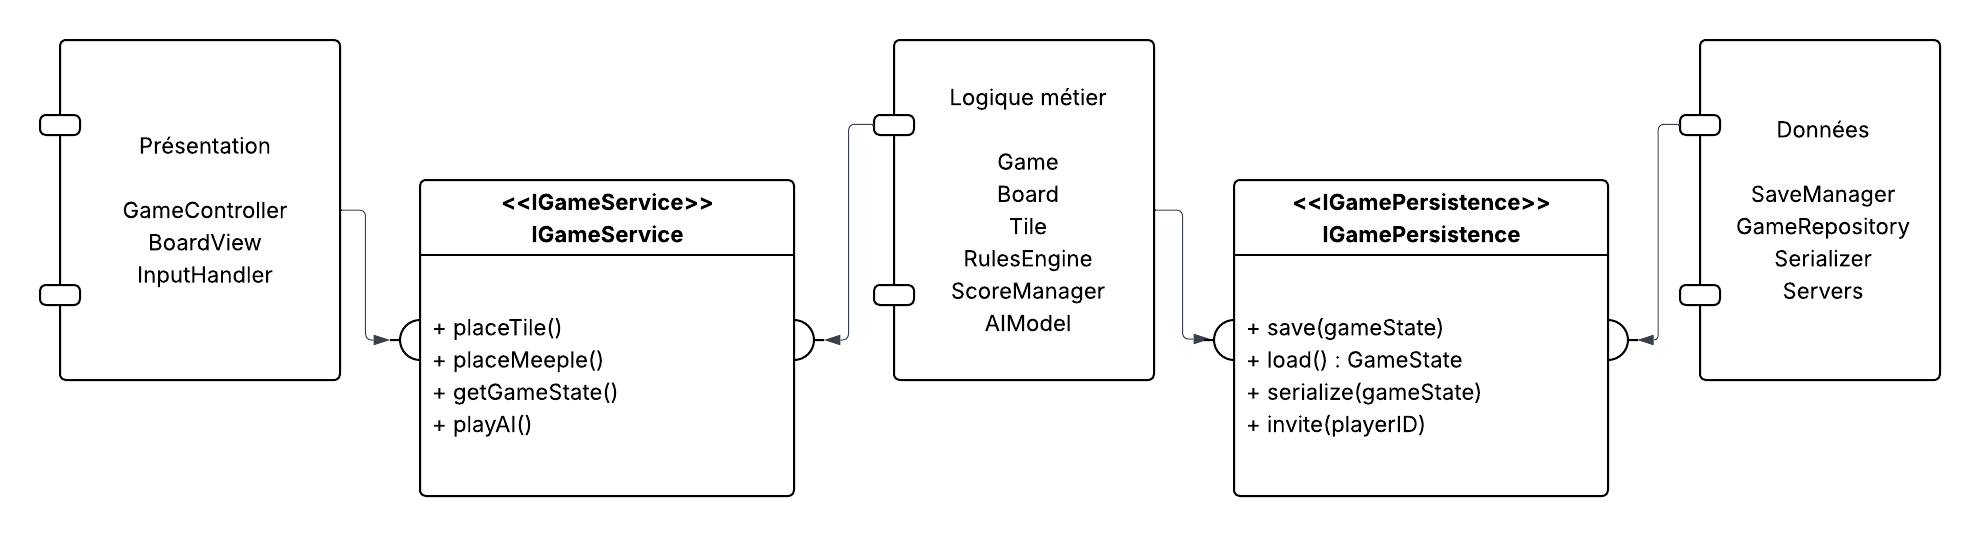
\includegraphics[width=1\textwidth]{images/UML_diagram.png}}
    \centering
    \caption{Diagramme UML du projet}\label{fig:UML_diagram}
\end{figure}

Ainsi, le module Présentation dépend uniquement du module Logique Métier, qu'il sollicite via des interfaces dédiées pour afficher l'état du jeu et transmettre les actions de l'utilisateur, sans accès direct aux données.
Le module Logique Métier dépend uniquement du module Données pour la persistance des informations, cette interaction étant réalisée au moyen d'interfaces de persistance abstraites.
Aucune dépendance directe n'existe entre la Présentation et les Données.

Cette organisation garantit une séparation claire des responsabilités et limite le couplage entre les composants.

\subsection{Interfaces principales}

Les interactions entre modules sont réalisées exclusivement via des interfaces bien définies.

Interface Présentation $\rightarrow$ Logique Métier

Exemples de services exposés :

{\normalsize
  \begin{minted}[frame=single]{python}
place_tile(tile, position)
place_meeple(position)
get_game_state()
is_game_over()
  \end{minted}
}



Ces interfaces permettent à la présentation d'agir sur le jeu sans connaître l'implémentation interne des règles.

Interface Logique Métier $\rightarrow$ Données

Exemples de services exposés :

{\normalsize
  \begin{minted}[frame=single]{python}
save_game(game_state)
load_game()
  \end{minted}
}




La logique métier délègue la persistance au module Données via ces interfaces abstraites.


\section{Explication approfondie}

Notre projet de Carcassonne en Python a été bien différent de ce que nous avions initialement prévu, notamment en raison de la complexité du jeu et des défis techniques rencontrés.
Dans cette section, nous allons expliquer en détail les différentes étapes de notre développement, les choix que nous avons faits ainsi que les difficultés que nous avons rencontrées pour deux fonctionnalités principales.


\subsection{Première fonctionnalité : Joueur artificiel}

Parmi les intelligences artificielles implémentées, nous avons développé l'algorithme MCTS (Monte Carlo Tree Search). Les fichiers correspondants à son implémentation se trouvent dans le module Business Logic, plus précisément dans le fichier \texttt{mcts\_player.py}.

Pour appliquer cet algorithme, nous avons représenté les nœuds de l'arbre à l'aide de la classe \texttt{MCTSNode}. Celle-ci contient l'état courant du jeu (\texttt{state}), son parent éventuel (\texttt{parent}), le coup ayant mené à ce nœud (\texttt{move}), le joueur associé à ce nœud (\texttt{player}), ainsi que le joueur MCTS à l'origine de son appel (\texttt{mcts\_player}). Elle inclut également la liste de ses enfants (\texttt{children}), les coups encore non explorés depuis ce nœud (\texttt{untried\_moves}), le nombre de visites (\texttt{visits}) et le score cumulé (\texttt{total\_reward}). Des accesseurs sont définis pour chacun de ces attributs, ainsi que deux méthodes dédiées à la mise à jour du nombre de visites et du score.

La classe \texttt{MCTSPlayer} centralise le déroulement complet de l'algorithme et construit progressivement l'arbre d'exploration via les \texttt{MCTSNode}. Elle inclut notamment l'état courant du jeu (\texttt{game}), les informations temporelles liées au tour de jeu de l'IA (à savoir le temps de départ, la durée maximale autorisée et le temps de fin : \texttt{start\_time}, \texttt{max\_time} et \texttt{end\_time}) afin d'interrompre l'algorithme si la limite est atteinte. Elle intègre également une fonction de sélection des enfants (\texttt{eval\_fn}), un modèle de sélection basé sur le machine learning (\texttt{ml\_model}), un booléen indiquant si ce modèle doit être utilisé comme fonction de sélection (\texttt{\_ml\_model\_attempted}), ainsi qu'une structure de stockage permettant d'enregistrer les scores au fil des simulations et d'en permettre la restauration pendant l'exécution de l'algorithme (\texttt{\_sim\_state\_stack}).

Le fonctionnement de l'algorithme repose sur la répétition de cinq étapes principales :
\begin{itemize}
  \item[$\bullet$] \textbf{Sélection :} à partir de la racine, on descend dans l'arbre en choisissant les enfants selon une fonction de sélection, jusqu'à atteindre un nœud à explorer.
  \item[$\bullet$] \textbf{Expansion :} un nouveau coup est sélectionné parmi ceux non encore explorés, ce qui crée un nouvel enfant.
  \item[$\bullet$] \textbf{Simulation :} une partie est simulée de manière aléatoire à partir de ce nouvel état.
  \item[$\bullet$] \textbf{Récompense :} le score final de la simulation est récupéré.
  \item[$\bullet$] \textbf{Rétropropagation :} les résultats sont propagés en remontant l'arbre jusqu'à la racine, en mettant à jour les statistiques des nœuds.
\end{itemize}

À l'issue de l'algorithme, le coup choisi correspond au nœud enfant de la racine présentant le meilleur score.

Les fonctions \texttt{play\_move\_for\_ai} et \texttt{undo\_for\_ai} permettent de simuler des coups sans altérer définitivement l'état réel du jeu. Lorsqu'un coup est joué via \texttt{play\_move\_for\_ai}, l'état courant (scores, meeples, structures du graphe, etc.) est sauvegardé avant application puis stocké dans une pile. À l'inverse, \texttt{undo\_for\_ai} restaure précisément cet état en annulant le dernier coup joué. Ce mécanisme garantit que chaque simulation reste indépendante et n'impacte jamais la partie réelle.

La fonction \texttt{get\_possible\_moves} génère l'ensemble des coups possibles à partir de l'état courant et de la tuile en main. Elle consiste à tester toutes les positions, rotations et placements de meeples possibles, puis à vérifier leur validité à l'aide de la fonction \texttt{check\_move} définie dans \texttt{rules\_manager.py}.

La sélection des nœuds dans l'arbre peut se faire via l'algorithme UCT (Upper Confidence Bound applied to Trees). Cette méthode équilibre exploitation (favoriser les coups déjà performants) et exploration (tester de nouvelles possibilités) grâce à un paramètre de pondération. Elle prend en compte le nombre de visites et les scores des nœuds, tout en priorisant les nœuds encore jamais explorés afin d'assurer une couverture suffisante de l'espace des coups possibles.

Une alternative à la méthode UCT consiste à utiliser une sélection guidée par le machine learning. Dans ce cas, un modèle Keras est chargé afin d'évaluer les coups possibles. Pour chaque enfant d'un nœud, un vecteur de caractéristiques est construit, incluant notamment le reward moyen, le nombre de visites, le score du joueur ou encore la présence d'un meeple. Le modèle prédit ensuite un score pour chaque coup et celui obtenant la meilleure évaluation est sélectionné. En cas d'indisponibilité du modèle, le système revient automatiquement à la méthode UCT.

Ce modèle de machine learning est entraîné à partir de données générées lors de simulations de parties. Pour chaque état exploré, des caractéristiques sont extraites et associées à un résultat, généralement le reward final ou une estimation de la qualité du coup. Ces données permettent d'entraîner un réseau de neurones (via Keras) capable de prédire la pertinence d'un coup en fonction de son contexte. Une fois entraîné, le modèle est sauvegardé dans un fichier et peut être rechargé pour guider la phase de sélection dans MCTS.

Les données utilisées pour l'entraînement sont stockées sous forme de fichiers JSON ou JSON Lines. Chaque entrée contient un vecteur de caractéristiques décrivant un état ou un coup, ainsi qu'une valeur cible représentant sa qualité, souvent le reward final ou une probabilité de victoire estimée. Le chargement de ces données est assuré par la fonction \texttt{\_load\_samples}, qui extrait une matrice de caractéristiques (chaque ligne correspondant à un coup) et un vecteur de cibles associées, puis les convertit en tableaux numériques exploitables via NumPy.

Le modèle adopté est un réseau de neurones de type perceptron multicouche (MLP), implémenté avec Keras. Il se compose d'une couche d'entrée adaptée au nombre de caractéristiques, suivie de deux couches cachées utilisant des fonctions d'activation ReLU, puis d'une couche de sortie produisant une valeur réelle. Cette dernière correspond à l'évaluation prédite du coup, avec une activation linéaire adaptée à une tâche de régression. L'entraînement consiste à ajuster les paramètres du réseau afin de minimiser l'écart entre les prédictions et les valeurs cibles, en utilisant la fonction de perte MSE (Mean Squared Error) ainsi que l'optimiseur Adam, reconnu pour sa stabilité et sa rapidité de convergence. L'apprentissage s'effectue sur plusieurs epochs avec un traitement des données par lots (batchs), ce qui améliore les performances globales.

Une fois entraîné, le modèle est sauvegardé au format \texttt{.keras}, incluant l'architecture et les poids du réseau. Il peut ainsi être rechargé ultérieurement sans nécessiter de nouvel entraînement. Lors de l'exécution de MCTS, ce modèle est chargé dynamiquement et utilisé pour évaluer les coups à partir de leurs caractéristiques. L'intégration avec MCTS est directe : les mêmes caractéristiques que celles utilisées lors de l'entraînement sont reconstruites en temps réel pour chaque nœud exploré (via \texttt{\_extract\_ml\_features}). Le modèle prédit alors un score pour chaque enfant, permettant d'orienter la sélection vers les coups les plus prometteurs. Cette approche offre une exploration plus informée que la méthode purement statistique UCT, tout en restant compatible avec celle-ci en cas d'absence de modèle.

\subsection{Seconde fonctionnalité : Jeu en réseau}

La partie concernant les besoins du serveur est découpée en deux sous-parties : le client, qui représente la personne au clavier, et le serveur, qui représente le serveur local de la machine. La partie serveur est quant à elle découpée en trois sous-parties :
\begin{itemize}
  \item [$\bullet$] \texttt{online\_communications}, qui représente les possibles réponses du serveur aux différents clients ;
  \item [$\bullet$] \texttt{games\_repository}, qui représente la base de données et les opérations sur celle-ci ;
  \item [$\bullet$] \texttt{server}, qui représente le fonctionnement global du serveur (gestion des clients, des parties et de l'état interne du serveur).
\end{itemize}

\subsubsection{Serveur}
La première fonction du serveur est \texttt{server\_start}. Cette fonction démarre le serveur en TCP sur un port donné en argument. Si aucun port n'est donné, le port 12345 sera utilisé par défaut. Suite à cela, un thread pour le serveur est créé et démarré sur la fonction \texttt{server\_running}.

La fonction \texttt{server\_running} permet d'accepter des connexions clients tant que le serveur tourne. De plus, un timer est mis en place pour envoyer périodiquement les informations nécessaires aux clients afin qu'ils puissent se connecter. Cela est fait par UDP broadcast toutes les 10 secondes. Cette fonction prend aussi en charge les lancements et fins de parties ainsi que les time-out des invitations de chaque client. Finalement, chaque socket de client accepté est dirigé sur son propre thread vers la fonction \texttt{handle\_client}.

Pour accomplir cette gestion, plusieurs fonctions internes sont utilisées. La première est \texttt{check\_all\_invitations\_timeout}, qui renvoie la liste des clients ayant reçu une invitation dont le délai de réponse est dépassé. La fonction \texttt{launch\_availables\_games} permet quant à elle de lancer toutes les parties pouvant l'être, c'est-à-dire les parties pour lesquelles les invitations ont toutes été résolues et le nombre de joueurs est correct. Conjointement, la fonction \texttt{clean\_finished\_games} se charge de nettoyer les parties terminées, tandis que \texttt{check\_clients\_timeout} vérifie si les clients ayant effectué une déconnexion inopinée ont dépassé leur délai de time-out.

Chaque socket de client est ensuite redirigé dans son propre thread vers la fonction \texttt{handle\_client}, qui se charge de la communication entre le serveur et un client. Si le client souhaite quitter, un message est envoyé à tous les clients du serveur. La commande \texttt{quit} est la seule commande qui peut être effectuée sans être enregistré auprès du serveur. Si le client n'est pas encore enregistré, la fonction \texttt{handle\_client\_registering} se charge de l'enregistrer, et différents messages sont envoyés en fonction de la réussite ou de l'échec de l'enregistrement. Dans le cas d'un échec, deux messages principaux peuvent être envoyés : soit le nom d'utilisateur est déjà pris, soit le client est sous un time-out pour déconnexion inopinée.

Une fois le client enregistré auprès du serveur, celui-ci traite les messages du client et envoie les réponses appropriées via la fonction \texttt{process\_message}, qui utilise la classe \texttt{online\_communications} afin de déterminer les réponses. La gestion de nombreuses erreurs est présente dans cette fonction, et quoi qu'il arrive, les structures de données du serveur seront mises à jour.

Les dernières fonctions notables du serveur sont les suivantes : \texttt{send\_to\_group} et \texttt{send\_to\_client}, qui permettent d'envoyer des messages respectivement à un groupe de joueurs ou à un joueur. On trouve également des accesseurs pour les différentes structures de données du serveur, ainsi que la fonction \texttt{server\_stop}, appelée aussi bien lors d'un arrêt normal que lors d'un arrêt brutal du serveur. Cette fonction nettoie toutes les ressources proprement.


\subsubsection{Client}
Le fichier \texttt{client.py} sert principalement à envoyer et recevoir des informations depuis le serveur auquel il est connecté.

La première fonction utilisée est \texttt{create\_default\_online\_player}. Elle se charge de créer un compte pour un serveur donné. Par défaut, il s'agit du serveur local. Toutefois, si un problème d'authentification survient sur un serveur externe, cette fonction permet de créer un compte spécifique pour ce serveur, en générant un nouveau nom d'utilisateur tout en conservant le même mot de passe.

La deuxième fonction rencontrée est \texttt{list\_available\_servers}. Elle écoute sur le port 12346 pour détecter les transmissions UDP broadcast des serveurs et constitue à partir de celles-ci une liste de serveurs disponibles. Tout serveur n'ayant pas envoyé de message depuis un certain temps est retiré de cette liste par la fonction \texttt{check\_servers\_last\_time\_sent}, qui vérifie la date de la dernière diffusion de chaque serveur.

Ensuite, la fonction \texttt{join\_server} permet de rejoindre un serveur figurant dans la liste des serveurs disponibles. Si aucun argument n'est fourni à cette fonction, elle récupérera les informations nécessaires auprès du serveur personnel, à condition que celui-ci figure dans la liste des serveurs disponibles ; sinon, aucune connexion ne sera établie. Lorsqu'une connexion est effectuée, un thread est créé côté client pour gérer la communication avec le serveur.

La fonction interne \texttt{\_receive\_loop} s'occupe de lire les messages tant que la connexion est active. Si elle reçoit un message du serveur indiquant un arrêt (\textit{shutdown}), la boucle se termine ; dans le cas contraire, les messages sont transmis à la fonction \texttt{handle\_server\_message}. Cette fonction sert à transmettre les messages du serveur au GUI si celui-ci est disponible. Elle se charge également d'automatiser certains comportements du client : par exemple, lorsqu'un client tente de se connecter pour la première fois et que le serveur renvoie un message indiquant que son nom d'utilisateur est déjà pris, la fonction offre au client la possibilité de modifier son nom d'utilisateur. En CLI, cette fonction affiche les messages du serveur sous une forme plus lisible.

Une autre fonction importante est \texttt{send\_to\_server}. Assez simple, elle transmet le message fourni en paramètre au serveur, selon le format suivant :

\begin{center}
    \texttt{username: message}
\end{center}

La fonction \texttt{connected\_to\_a\_server} est une fonction servant la logique interne du client. Enfin, la fonction \texttt{disconnect} prend en charge les déconnexions brutes et normales et se charge de nettoyer toutes les ressources de la session qui ne sont pas des ressources de la base de données. Il existe également la fonction \texttt{register\_message\_visitor} qui utilise l'idée du design pattern visitor afin de pouvoir capturer les messages envoyés par le serveur pour les transmettre au GUI.


\subsubsection{Online\_communications}

La classe \texttt{OnlineCommunication} se charge de retourner les réponses appropriées aux commandes et d'effectuer les opérations demandées si elles peuvent l'être. Ses fonctions peuvent être séparées en deux catégories : les commandes spécifiques au serveur et les commandes spécifiques au jeu.

La commande \texttt{quit} demande à la base de données d'effectuer les modifications nécessaires pour déconnecter le client et renvoie ensuite le message correspondant. La commande \texttt{server status} transmet les informations pertinentes concernant le serveur. La commande \texttt{new~...}, quant à elle, envoie des invitations aux joueurs disponibles figurant dans la liste d'identifiants fournie. Si aucun joueur n'est disponible, une réponse appropriée est renvoyée.

La plupart des commandes dépendent de l'état du serveur et/ou de la base de données. Toutes les commandes liées au jeu ne produiront aucun effet et renverront un message adapté si le joueur n'est pas actuellement dans une partie. Enfin, la commande \texttt{ping} mérite une mention spéciale : elle se contente de renvoyer \texttt{pong}.

\subsubsection{Base de données}

La base de données constitue un élément central du serveur. Presque toutes les opérations importantes y passent, que ce soit pour récupérer des informations, en créer de nouvelles, les modifier, ou plus rarement les supprimer. La classe \texttt{games\_repository} est conçue de manière à ce que le serveur et la logique métier n'aient pas à connaître la structure interne de la base de données.

Toutes les opérations sur la base de données reposent sur deux types de transactions : les transactions \textit{query}, qui sont des transactions de sélection de données, et les transactions \textit{non query}, qui sont des transactions de modification des n-uplets. Ces opérations sont protégées contre toute injection de code SQL par des utilisateurs malveillants.

Pour répondre aux besoins de Carcassonne, plusieurs tables ont été créées. La première, et l'une des plus importantes, est la table des joueurs. Chaque joueur y possède un identifiant unique généré automatiquement par la base de données. La table contient également le nom d'utilisateur principal et le mot de passe. Le statut du joueur est inclus pour gérer correctement les événements et peut prendre l'une des quatre valeurs suivantes : \texttt{idle}, \texttt{away}, \texttt{waitgame} ou \texttt{ingame}, représentant les différents états possibles du joueur. Le numéro de groupe du joueur est également présent et est initialement à \texttt{null}. Enfin, deux booléens sont utilisés : l'un indique si le joueur est connecté et l'autre s'il est un client courtois, c'est-à-dire un client qui quitte le serveur correctement.

Pour représenter les groupes de joueurs dans chaque partie, la table \texttt{groups} contient l'identifiant auto-généré du groupe, le nombre de joueurs dans celui-ci et l'identifiant de l'hôte. La table \texttt{scoreboard} est plus simple : elle stocke pour chaque joueur son identifiant, son nombre de victoires et de défaites. La table \texttt{current\_games} conserve les parties en cours avec l'identifiant auto-généré de la partie, son nom et le groupe associé.

L'une des tables les plus importantes pour la gestion des parties est la table \texttt{pending\_invitations}. Chaque invitation y possède un identifiant auto-généré, l'identifiant du groupe concerné, l'identifiant du joueur invité et le statut de l'invitation, qui peut être soit \texttt{waiting} soit \texttt{accepted}. La date d'envoi de l'invitation est également enregistrée afin de gérer le temps maximum de réponse.

Pour gérer les conflits de noms d'utilisateurs entre différents serveurs, la table \texttt{usernames} a été créée. Elle contient l'adresse du serveur et le nom d'utilisateur associé. Si un serveur n'est pas présent dans cette table, le nom d'utilisateur principal est utilisé à condition qu'il ne soit pas déjà pris sur ce serveur, ou la phase d'enregistrement n'a pas encore eu lieu. Cette table est la seule à contenir des données propres au propriétaire de l'ordinateur. Enfin, la table \texttt{timeouts} enregistre les identifiants des joueurs qui se sont déconnectés de manière inattendue ainsi que la date à laquelle cette déconnexion a été constatée par le serveur.

\section{Revue critique du projet}

Nous avons fait face à plusieurs défis au cours de ce projet notamment en ce qui concerne la complexité du jeu et la mise en œuvre de l'intelligence artificielle.
Dans un premier temps, nous allons discuter de la complétion du cahier des charges du projet. Ensuite, nous analyserons les performances obtenues ainsi que les limites de notre implémentation. Enfin, nous terminerons par une discussion sur les pistes d'amélioration possibles pour notre projet.


\subsection{Cahier des charges}

Dans cette section, nous allons discuter de la manière dont nous avons respecté le cahier des charges du projet en analysant chaque partie et en expliquant ce qui a été réalisé et ce qui n'a pas été fait.

\subsubsection{Généralités}

Cette première partie du projet a été globalement respectée. Des tests 
ont été mis en place tout au long du développement afin de vérifier le 
bon fonctionnement du code et de s'assurer que les différentes 
fonctionnalités étaient correctement implémentées. Avant le rendu, nous 
avons également vérifié la compatibilité des bibliothèques utilisées 
avec les exigences du cahier des charges.

Grâce à cette approche, le projet atteint une couverture globale 
d'environ 80\% ce qui constitue un résultat conforme aux exigences 
du cahier des charges.


\subsubsection{Besoins généraux}

Cette partie a été relativement simple à respecter.
La principale difficulté a toutefois résidé dans la mise en place du 
fichier de configuration du besoin F2 en lien avec l'ensemble des fonctionnalités 
supplémentaires ajoutées au fil du projet.
Un problème subsiste cependant : le cahier des charges stipule que le 
fichier de configuration doit être lu au démarrage et ses options utilisées 
par défaut. Or, une fois ce fichier présent, il n'est plus possible de 
revenir aux options par défaut du programme sans modifier manuellement 
le fichier. Une commande dédiée à la réinitialisation des options par 
défaut aurait été nécessaire pour pallier ce manque.

\subsubsection{Options au lancement}

Les besoins portaient 
principalement sur des options de lancement relativement faciles à 
implémenter. Il a néanmoins fallu intégrer différents modes de jeu 
comme le mode \textit{Blitz} ou \textit{Contest} (F6 et F7) ainsi que l'extension 
\textit{The River} (F10). Ces éléments ont été réalisés en fin de projet une 
fois les fonctionnalités de base implémentées ce qui a facilité leur 
intégration.

Une difficulté particulière a cependant été rencontrée lors de 
l'implémentation de \textit{The River}, concernant la règle de virage. 
En effet, cette règle impose des contraintes sur l'orientation des tuiles 
rivière afin d'éviter que la rivière ne forme une boucle ce qui s'est 
révélé non trivial à vérifier lors du placement des tuiles.

Nous pouvons également mentionner les algorithmes de mélange de tuiles 
et leurs tests statistiques, détaillés en section \ref{subsubsec:melange}.



\subsubsection{Gestion du jeu}

La gestion des règles de base du jeu a constitué la première grande 
étape du projet, mais aussi l'une des premières difficultés majeures. 
Les règles de Carcassonne sont en effet relativement complexes à 
implémenter : connectivité des tuiles, conditions de placement des 
pions, calcul du score — chacun de ces aspects a nécessité une grande 
rigueur afin de garantir une implémentation correcte.

Le placement des tuiles et des pions a été relativement simple à 
traiter, notamment grâce à une bonne modélisation du plateau de jeu 
et des tuiles via le module \textit{graph}. En revanche, la gestion 
du score a représenté un défi majeur. Elle a nécessité la mise en place 
de composantes connexes, en particulier pour les champs pouvant 
s'étendre entre routes et cités, dont la délimitation s'est révélée 
particulièrement délicate à formaliser. Cette partie a été source de 
nombreux bugs et a significativement ralenti l'avancement du projet.

\subsubsection{Command Line Interface (CLI)}

Le CLI a été relativement simple à implémenter, notamment grâce à la 
bibliothèque \textit{readline} de Python, qui facilite la saisie des 
commandes et a permis de répondre aisément à deux besoins principaux : 
l'édition de la commande en cours et la gestion de l'historique des 
commandes tapées. Il a toutefois été nécessaire de développer des 
fonctions spécifiques pour l'auto-complétion des commandes et de leurs 
arguments afin de satisfaire le besoin F19.

Une amélioration notable resterait la mise en place d'un design pattern 
dédié à la gestion des commandes (besoin F15). Une telle approche aurait 
permis de mieux structurer le système dès le départ et d'en faciliter 
l'évolution, notamment lors de l'implémentation des commandes dans le 
GUI, où l'absence de cette structure s'est fait ressentir.


\subsubsection{Format de sauvegarde}

Cette partie a été développée progressivement au fil de l'avancement du projet. 
Nous avons d'abord mis en place une sauvegarde basique de l'état du jeu, avant d'y ajouter des fonctionnalités complémentaires, telles que la gestion du format de l'historique et la conformité avec le fichier de configuration.
Elle inclut également la représentation du plateau de jeu, qui s'est révélée relativement simple à implémenter, celui-ci étant peu complexe à exprimer sous forme textuelle.


\subsubsection{Structures de données}

La mise en place d'un graphe pour représenter le plateau de jeu a été la première étape du projet.
Ce graphe nous a permis de gérer efficacement les différentes connectivités entre les tuiles notamment pour la gestion du score des champs en utilisant des composantes connexes.
Cependant, cette implémentation précoce a également été à l'origine de nombreuses difficultés et de bugs par la suite. En particulier, l'absence d'une véritable classe Tile, où les éléments du graphe sont en réalité modélisés comme des Vertex, a complexifié la gestion du code notamment lors de l'implémentation du GUI.


\subsubsection{Graphical User Interface (GUI)}

L'implémentation du GUI a été, en parallèle de l'intelligence 
artificielle, la partie la plus longue du projet. Le principal défi a 
résidé dans la dépendance du GUI vis-à-vis des autres fonctionnalités 
du projet : il a en effet fallu attendre que les différentes composantes 
soient suffisamment stables pour pouvoir les intégrer dans l'interface 
graphique. Le GUI s'est également révélé plus complexe à développer que 
le CLI, nécessitant la mise en place de nombreux éléments graphiques 
tels que des menus, des boutons, ainsi que l'affichage des tuiles et 
des meeples.

Une difficulté technique notable a été la gestion du placement des 
tuiles sur le plateau. Le GUI repose sur un système de coordonnées 
$(x, y)$ pour représenter les positions, tandis que le module de logique 
métier utilise une référence par tuile et orientation. Il a donc fallu 
établir une correspondance entre ces deux représentations. Pour cela, 
nous avons mis en place une fonction permettant de retrouver la tuile 
voisine d'une position $(x, y)$ donnée sur le plateau, utilisée ensuite 
comme entrée pour le \textit{play\_move} du module de logique métier.

Malgré ces avancées, certaines améliorations restent envisageables, 
notamment concernant l'adaptabilité du plateau à la taille de la fenêtre 
et la gestion exhaustive des erreurs utilisateur, pour rendre le GUI 
pleinement cohérent avec l'ensemble des besoins du projet.

\subsubsection{Joueur artificiel}

La partie concernant les joueurs artificiels a été la plus complexe du projet. En effet, comme abordé dans la section \ref{subsec:minimax}, Carcassonne est un jeu à la fois stochastique et à information parfaite
ce qui rend l'implémentation de Minimax inutilisable dans sa forme classique.
Il a fallu ainsi implémenter une version adaptée de Minimax avec des noeuds chance pour prendre en compte de la pioche des tuiles. 
Cette approche correspond à l'algorithme Expectimax, une extension de Minimax pour les jeux stochastiques.
Cependant, l'implémentation de cet algorithme s'est avérée très complexe et a été source de nombreux bugs, notamment en ce qui concerne la gestion des noeuds chance et la mise en place de fonctions d'évaluation heuristiques adaptées à ce jeu.


\subsubsection{Jeu en réseau}


La partie la plus chronophage a été la gestion du serveur côté GUI. 
Plus précisément, il a fallu permettre au GUI d'afficher les messages 
envoyés par le serveur, pour laquelle nous avons mis en place le design 
pattern Visitor, afin que le GUI puisse traiter et afficher ces messages 
sans établir de lien direct entre les deux composants.

La partie la plus complexe a quant à elle été la gestion des différentes 
commandes envoyées par le serveur. En effet, la base de données ayant 
évolué tout au long du projet, le comportement associé à chaque commande 
a dû être régulièrement revu. De plus, la base de données se devant de 
refléter fidèlement l'état réel du serveur, toute modification doit se 
répercuter de manière cohérente entre les deux, ce qui complexifie 
significativement la gestion des commandes.

Par ailleurs, la gestion des interruptions abruptes du serveur ou du 
client a été une source de nombreux bugs, nécessitant la mise en place 
de fonctions de nettoyage afin d'éviter les fuites de ressources et la 
corruption de la base de données.

Cependant, les besoins F39 et F40 n'ont été que partiellement réalisés 
côté GUI : si la réception et l'affichage des messages serveur 
fonctionnent correctement, le lancement d'une nouvelle partie via la 
commande \texttt{new} depuis le GUI reste non opérationnel. Cette 
fonctionnalité est en revanche pleinement prise en charge dans le CLI.

\subsection{Performance}

Cette section a pour objectif d’évaluer empiriquement les performances des différentes composantes du projet, en particulier les intelligences artificielles et certains choix algorithmiques.
Nous analysons les résultats obtenus à travers plusieurs expérimentations afin d’identifier les comportements observés, leurs limites ainsi que les pistes d’amélioration possibles.

\subsubsection{IA}
\label{subsubsec:iaperfo}

\begin{table}[h]
\centering
\begin{tabular}{lcccc}
\hline
\textbf{IA} & \textbf{Wins (incl. ties)} & \textbf{Win rate} & 
\textbf{Avg score} & \textbf{Avg place} \\
\hline
Iterative  & 9 & 60.0\% & 22.0 & 1.63 \\
Random     & 3 & 20.0\% & 15.1 & 3.43 \\
MCTS\_ML   & 2 & 13.3\% & 14.3 & 3.20 \\
Minimax    & 2 & 13.3\% & 14.3 & 3.33 \\
MCTS\_UCT  & 1 &  6.7\% & 14.7 & 3.40 \\
\hline
\end{tabular}
\caption{Comparaison des performances des différentes IA sur 15 parties 
mixtes, chaque partie incluant une IA de chaque type.}
\end{table}

Ce tableau présente les performances des différentes intelligences 
artificielles sur 15 parties mixtes. L'IA Iterative domine nettement 
avec un taux de victoire de 60\% et une position moyenne de 1.63, tandis 
que les autres IA, notamment les variantes MCTS, obtiennent des 
performances significativement plus faibles dans ce contexte compétitif.

Ce résultat est d'autant plus surprenant que des expérimentations 
préalables montrent que les IA basées sur MCTS atteignent entre 60\% 
et 80\% de taux de victoire lorsqu'elles sont évaluées contre des IA 
aléatoires. Ces performances ont été mesurées sous différentes 
contraintes de temps de calcul :
\begin{itemize}
    \item 1 seconde : environ 25 itérations par tour (UCT) contre 15 (ML)
    \item 5 secondes : environ 112 itérations (UCT) contre 68 (ML)
\end{itemize}

Ce contraste met en évidence un point important : une IA performante en 
environnement contrôlé ne garantit pas de bonnes performances en contexte 
multi-agents compétitif. Plusieurs hypothèses peuvent expliquer ce 
phénomène. D'une part, les simulations MCTS reposent sur des modèles 
adverses simplifiés, souvent aléatoires, ce qui les rend moins robustes 
face à des stratégies variées. D'autre part, le coût computationnel élevé 
des simulations, qui impliquent de rejouer toute la logique du jeu, limite 
le nombre d'itérations réalisables et donc la qualité des décisions prises. 
Enfin, les variantes MCTS implémentées (UCT et ML) peuvent ne pas être 
optimalement adaptées à ce type de jeu ou à ce format multi-joueurs.

\subsubsection{Algorithme de mélange des tuiles}
\label{subsubsec:melange}

Un point plus technique concerne les algorithmes de mélange des tuiles dont la validation a nécessité deux niveaux de tests. 
Le premier repose sur des tests fonctionnels déterministes : pour un paquet initial donné, un même algorithme et une même graine doivent produire un résultat identique. 
Nous vérifions également que le mélange conserve exactement le multiensemble des tuiles, sans perte, duplication ni altération. 
Dans le cas du paquet « rivière », une contrainte supplémentaire impose que la tuile spéciale finale reste en dernière position. 
Ces tests garantissent la reproductibilité et l'intégrité des structures de données mais ne permettent pas à eux seuls d'évaluer la qualité statistique du mélange.

Pour analyser l'uniformité des algorithmes, nous avons étudié un cas simplifié composé de trois tuiles distinctes.
Ce choix est justifié par le fait que le paquet réel contient des doublons, ce qui rend l'analyse des permutations plus difficile, tandis qu'un paquet de trois éléments permet une étude exhaustive et exacte. 
Avec Fisher-Yates, l'algorithme effectue successivement un choix parmi 3 possibilités puis un choix parmi 2 possibilités, soit $3 \times 2 = 6$ trajectoires, exactement le nombre de permutations possibles. 
L'énumération complète montre que chacune des 6 permutations est obtenue une seule fois : la distribution est donc uniforme. 
À l'inverse, l'algorithme naïf effectue 3 échanges avec à chaque fois 3 choix possibles, soit $3^3 = 27$ trajectoires. 
L'énumération exhaustive donne alors des effectifs $(5,5,5,4,4,4)$ pour les 6 permutations, au lieu d'une répartition uniforme. 
Cela montre que plusieurs suites d'échanges conduisent plus souvent à certaines permutations qu'à d'autres.
Ces résultats confirment les propriétés théoriques des deux méthodes : Fisher\-Yates est uniforme lorsque les indices sont tirés uniformément, alors que l'algorithme naïf est structurellement biaisé. 
Nous avons donc retenu Fisher\-Yates comme algorithme par défaut, tandis que l'algorithme naïf est conservé à des fins de comparaison expérimentale.


\subsection{Limites et bugs}

Toutefois, malgré nos efforts pour implémenter correctement les différentes fonctionnalités du projet, nous avons rencontré de nombreux bugs et limitations au cours du développement.

\subsubsection{Limites}
\begin{itemize}
  \item [$\bullet$] Nous n'avons pas traité le cas d'une tuile impossible 
  à placer ce qui peut survenir dans certaines configurations de jeu. 
  Dans ce cas, le comportement du programme n'est pas défini : la partie 
  peut se bloquer sans message d'erreur explicite pour le joueur.
  \item [$\bullet$] La taille du plateau de jeu dans le GUI est fixe et 
  ne s'adapte pas dynamiquement à la taille de la fenêtre. Ainsi, si la 
  fenêtre est agrandie, les éléments de l'interface tels que les boutons 
  s'ajustent correctement, mais le plateau de jeu reste de taille fixe, 
  créant un déséquilibre visuel et une expérience utilisateur sous-optimale.
  \item [$\bullet$] Les fonctions d'évaluation heuristiques utilisées par 
  les IA ne modélisent pas certaines stratégies avancées, comme le blocage 
  adverse ou la gestion optimale des meeples restants. Cela limite leur 
  efficacité en contexte compétitif multi-joueurs, comme l'illustrent les 
  résultats présentés en section \ref{subsubsec:iaperfo}.
  \item [$\bullet$]  Un certain nombre de constantes du projet ne sont pas 
  centralisées et sont dispersées à travers les différents modules ce qui 
  nuit à la maintenabilité du code. En effet, toute modification d'une 
  valeur nécessite de retrouver et mettre à jour chaque occurrence 
  manuellement, augmentant ainsi le risque d'incohérences et d'erreurs 
  difficiles à détecter.
  \item [$\bullet$]  Le serveur ne semble fonctionner correctement que dans 
  l'environnement du Cremi. En effet, les tests effectués en réseau local 
  n'ont pas été concluants, suggérant que le serveur repose sur des 
  configurations réseau spécifiques à cet environnement. Cela constitue 
  une limitation importante quant à la portabilité du mode réseau du projet.
  \item [$\bullet$] Certaines spécifications du cahier des charges manquent 
  de clarté ce qui nous a conduits à interpréter et implémenter ces besoins 
  de manière intuitive, en adoptant la solution qui nous semblait la plus 
  logique. Ces choix d'interprétation peuvent ainsi ne pas correspondre 
  exactement aux attentes initiales du projet.
  C'est notamment le cas du 
  besoin F39 concernant le mode daemon du serveur, dont la spécification 
  est restée floue malgré des échanges avec les chargés de TD, et que nous 
  avons donc implémenté selon notre propre compréhension.
  De même, le besoin 
  F10 relatif à l'extension \textit{The River} a fait l'objet d'échanges 
  avec les chargés de TD dont les attentes semblaient différer de notre 
  implémentation, laissant penser que notre interprétation pourrait être 
  à revoir.

  \item [$\bullet$] 
\end{itemize}


\subsubsection{Bugs}

\begin{itemize}
  \item [-] Les besoins F39 et F40 concernant les fonctionnalités avancées du serveur sont pleinement fonctionnels dans le CLI, mais partiellement implémentés dans le GUI. 
  En particulier, la commande new permettant de lancer une nouvelle partie depuis le GUI n'est pas opérationnelle : le message est bien envoyé au serveur mais la réponse n'est pas correctement traitée et affichée côté GUI. 
  Cela s'explique par la complexité du pattern Visitor mis en place, qui n'a pas pu être étendu à temps à l'ensemble des types de messages du serveur.
  \item [-] 
\end{itemize}
\subsection{Perspectives d'amélioration}

Une fois le projet complété, nous avons identifié plusieurs pistes 
d'amélioration, que ce soit au niveau de l'architecture du code, de 
l'implémentation de certaines fonctionnalités ou de l'extensibilité 
du projet.

\subsubsection*{Architecture et qualité du code}

L'amélioration la plus évidente concerne l'organisation générale du code. 
Un manque de prévoyance dans l'architecture initiale a conduit à des choix 
d'implémentation qui ont rendu certaines parties du projet difficiles à 
maintenir et à faire évoluer. Cela s'est illustré notamment lors de la 
restructuration des fichiers \textit{game.py} et \textit{gui.py}, qui 
dépassaient chacun les 1000 lignes et concentraient trop de 
responsabilités distinctes. Nous avons tenté de remédier à ce problème 
au fil du développement, mais avons parfois dû faire des compromis pour 
avancer dans les délais.

Une meilleure réflexion en amont sur l'architecture du projet aurait 
permis d'éviter ces écueils. Par exemple, la mise en place d'un design 
pattern dédié à la gestion des commandes aurait structuré davantage le 
système et facilité l'implémentation des commandes dans le GUI. De même, 
une centralisation des constantes dès le début du projet aurait amélioré 
la cohérence et la maintenabilité de l'ensemble du code.

\subsubsection*{Fonctionnalités et extensibilité}

Sur le plan fonctionnel, plusieurs aspects pourraient être améliorés.
La gestion des cas limites, comme celui d'une tuile impossible à placer,
mériterait d'être traitée explicitement afin de garantir un comportement
défini dans toutes les situations. Cette même rigueur pourrait être
appliquée à d'autres composantes du projet : la robustesse du serveur
face à des situations réseau inattendues, l'expérience utilisateur du
GUI notamment via un plateau adaptatif et une meilleure gestion des
erreurs, ou encore les performances de nos IA grâce à des fonctions
d'évaluation plus élaborées modélisant des stratégies avancées comme
le blocage adverse ou la gestion optimale des meeples.

Nous avons ainsi réussi à implémenter un projet fonctionnel répondant 
à une grande partie des besoins du cahier des charges. Les améliorations 
restantes relèvent principalement de la qualité du code, de la robustesse 
de certaines fonctionnalités et de l'expérience utilisateur, et ne 
remettent pas en cause le bon fonctionnement général du projet.

\subsection{Utilisation de l'IA}


Tout au long du projet, nous avons eu recours à des outils d'intelligence 
artificielle pour diverses tâches, que ce soit pour la mise en place d'un 
code de base, l'amélioration de la qualité du code ou l'affinement de 
certaines fonctionnalités. Cela nous a permis d'avancer plus rapidement 
et efficacement, tout en développant un regard critique sur les forces 
et les limites de chaque outil.

Nous avons largement utilisé l'extension \textit{GitHub Copilot} de 
Visual Studio Code, qui s'est révélée particulièrement efficace pour 
les tâches répétitives et bien délimitées, comme la génération de 
fonctions utilitaires ou la complétion de blocs de code dont la 
structure était déjà claire. En revanche, ses suggestions se sont 
montrées moins pertinentes pour des problèmes nécessitant une 
compréhension globale de l'architecture du projet, produisant parfois 
du code fonctionnel en apparence mais incohérent avec le reste du 
système.

Pour des problématiques plus complexes, nous avons eu recours à 
\textit{ChatGPT} et \textit{Claude}, notamment pour l'implémentation 
de fonctionnalités telles que la mise en place du design pattern Visitor 
pour l'affichage des réponses du serveur dans le GUI. Ces modèles se 
sont révélés utiles pour structurer une approche sur des problèmes 
architecturaux ou pour expliquer des concepts. Toutefois, nous avons 
constaté leurs limites lorsque le contexte du projet devenait trop 
volumineux : les suggestions proposées étaient alors déconnectées des 
choix d'implémentation existants et nécessitaient un travail 
d'adaptation important, voire introduisaient de nouveaux bugs.

Enfin, l'IA a également contribué à l'amélioration de ce rapport, en 
nous aidant à structurer nos idées, à formuler nos analyses de manière 
plus claire et concise, et à corriger les fautes d'orthographe et de 
grammaire.

\section{Liste des besoins}

\begin{longtable}{|c|l|c|}
\hline
\textbf{Besoin} & \textbf{Description du besoin} & \textbf{Statut} \\
\hline
\endfirsthead

\hline
\textbf{Besoin} & \textbf{Description du besoin} & \textbf{Statut} \\
\hline
\endhead

F1 & Lancement du programme & Non fait \\ \hline
F2 & Fichier de configuration & Non fait \\ \hline
F3 & Internationalisation (i18n) & Non fait \\ \hline
F4 & Interface en ligne de commande & Non fait \\ \hline
F5 & Interface graphique & Non fait \\ \hline
F6 & Mode blitz & Non fait \\ \hline
F7 & Mode contest & Non fait \\ \hline
F8 & Graine aléatoire & Non fait \\ \hline
F9 & Mélange des tuiles & Non fait \\ \hline
F10 & Options spécifiques & Partiel \\ \hline

F11 & Gestion des règles & Non fait \\ \hline
F12 & Gestion des erreurs utilisateur & Non fait \\ \hline
F13 & Gestion du undo/redo & Non fait \\ \hline
F14 & Gestion des conseils & Non fait \\ \hline

F15 & Shell interactif & Non fait \\ \hline
F16 & Proposer de sauvegarder avant quitter & Non fait \\ \hline
F17 & Édition de la commande en cours & Non fait \\ \hline
F18 & Historique des commandes tapées & Non fait \\ \hline
F19 & Complétion des commandes & Non fait \\ \hline
F20 & Notation des coups & Non fait \\ \hline

F21 & Sauvegarde et restauration d'une partie & Non fait \\ \hline
F22 & Commentaires dans la sauvegarde & Non fait \\ \hline
F23 & Format des paramètres du jeu & Non fait \\ \hline
F24 & Format du plateau de jeu & Non fait \\ \hline
F25 & Format de l'historique & Non fait \\ \hline

F26 & Module \textit{graph} & Non fait \\ \hline
F27 & Algorithmes de manipulation des graphes & Non fait \\ \hline

F28 & Menus de l'application & Non fait \\ \hline
F29 & Raccourcis clavier & Non fait \\ \hline
F30 & Drag'n'drop & Non fait \\ \hline

F31 & Temps de réflexion borné & Non fait \\ \hline
F32 & Minimax avec $\alpha$$\beta$-pruning & Non fait \\ \hline
F33 & Fonctions d'évaluation pour Minimax & Non fait \\ \hline
F34 & Approfondissement itératif de Minimax & Non fait \\ \hline
F35 & Profondeur de recherche de Minimax & Non fait \\ \hline
F36 & Monte Carlo Tree Search (MCTS) & Non fait \\ \hline
F37 & Fonction de sélection par Machine Learning & Non fait \\ \hline

F38 & Découverte de serveurs et connexion client-
serveur basique & Non fait \\ \hline
F39 & Serveur multi-clients et gestion de parties & Non fait \\ \hline
F40 & Système d'invitations et gestion avancée des
joueurs & Non fait \\ \hline

\end{longtable}


%------------------------------------------------------------------------------
%	BIBLIOGRAPHY
%------------------------------------------------------------------------------

\nocite{*}
\bibliographystyle{plain}
\bibliography{bibliography}

\end{document}
